\documentclass[11pt, a4paper, oneside, article]{memoir}
% Setting for memoir
% Set the margins of the document
\setlrmarginsandblock{2cm}{2cm}{*}
\setulmarginsandblock{2cm}{*}{1}
\checkandfixthelayout
%\OnehalfSpacing
\captionnamefont{\bfseries\small}
\captiontitlefont{\small}
\usepackage{calc}
\newif\ifNoChapNumber
\makechapterstyle{proposal}{%
\renewcommand{\chapterheadstart}{\vskip 1\baselineskip\medskip}
\renewcommand{\chapnamefont}{\normalfont\large\scshape}
\renewcommand{\chapnumfont}{\bfseries\LARGE\scshape}
\renewcommand{\chaptitlefont}{\normalfont\Large\scshape}
\renewcommand\chapternamenum{}
\renewcommand\printchaptername{}
\renewcommand\printchapternum{}
\renewcommand\printchaptertitle[1]{%
  \begin{tabular}{@{}p{1cm}|!{\quad}p{\textwidth-1cm-2em-4\tabcolsep }}
    \ifNoChapNumber\relax\else\chapnumfont \thechapter\fi
    & \chaptitlefont ##1
  \end{tabular}
  \NoChapNumberfalse}
\renewcommand\printchapternonum{\NoChapNumbertrue}
\renewcommand{\afterchaptertitle}{\par\nobreak\medskip\hrule\vskip 1\baselineskip}
}
\chapterstyle{proposal}
\setsecheadstyle{\normalfont\Large\scshape}
%\DisemulatePackage{setspace}            % Make sure package is not ignored
%\usepackage[onehalfspacing]{setspace}   % Set the line spacing of the document
%
\usepackage[german, english]{babel}     % Language setting
\usepackage[utf8]{inputenc}
\usepackage[usenames,dvipsnames]{xcolor}
\usepackage{graphicx}
\usepackage{wrapfig}                    % Wrapping text around figures
%\usepackage{subfigure}                 % Doesn't work with memoir class
\newsubfloat{figure}% Allow subfloats in figure environment
\usepackage{amsmath}                    % Advanced mathsymbols
\usepackage{chemformula}                % Chemical formulas
%\usepackage{pgfgantt}                   % GANTT charts
\usepackage[shortlabels]{enumitem}
\usepackage[colorlinks=false,linkcolor=black,urlcolor=black,bookmarksopen=true]{hyperref}
\usepackage{bookmark}
% Abbreviation glossary
\usepackage[acronym,nogroupskip,nonumberlist,toc]{glossaries}
\setglossarystyle{index}
\makeglossaries                         % Generate the glossary

% Bibliography with biblatex
\usepackage[citestyle=alphabetic,bibstyle=authoryear,citestyle=authoryear,maxbibnames=100,maxcitenames=1,sorting=nty,backend=biber]{biblatex}
\addbibresource[location=local, datatype=bibtex]{atmo.bib}

\usepackage{csquotes, xpatch}
\usepackage{etex, etoolbox, keyval, ifthen, url} % Needed for chicago-style citations

\usepackage[most]{tcolorbox}

%textmarker style from colorbox doc
\tcbset{textmarker/.style={%
        enhanced,
        parbox=false,boxrule=0mm,boxsep=0mm,arc=0mm,
        outer arc=0mm,left=6mm,right=3mm,top=7pt,bottom=7pt,
        toptitle=1mm,bottomtitle=1mm,oversize}}
% define new colorboxes
\newtcolorbox{importantBox}{textmarker,
    borderline west={6pt}{0pt}{blue},
    colback=blue!10!white}
% define commands for easy access
\newcommand{\important}[1]{\begin{importantBox} #1 \end{importantBox}}

\chapterstyle{proposal}             % Set style for memoir, bringhurst
\graphicspath{{pictures/}}              % Set graphics path

%DOCUMENT%
\begin{document}
\setlength{\baselineskip}{15pt}         % 15-20 pt

%Term definitions
% Standard command
%\gls{⟨label⟩}
% Capitalize first letter
%\Gls{⟨label⟩}
% Pluralize term
%\glspl{⟨label⟩}
%Capitalize and pluralize term
%\Glspl{⟨label⟩}

%\newacronym{}{}{}

% Acronyms
\newacronym{voc}{VOC}{Volatile Organic Compound}
\newacronym{bvoc}{BVOC}{Biogenic Volatile Organic Compound}
\newacronym{et}{ET}{evapotranspiration}
\newacronym{npp}{NPP}{Net Primary Production}
\newacronym{odina}{ODINA}{Ozone Damage Interference on Nutrient Allocation}
\newacronym{cuo}{CUO}{Cumulative Uptake of Ozone}
\newacronym{cesm}{CESM}{Community Earth System Model}
\newacronym{clm}{CLM}{Community Land Model}
\newacronym{cam}{CAM}{Community Atmosphere Model}
\newacronym{fun}{FUN}{Fixation and Update of Nitrogen}


\frontmatter
\tableofcontents*

\mainmatter
\chapter{Research context}
\label{c:context}
\section{Review of state of the field}
\label{sec:review}

\begin{wrapfigure}[14]{R}[0pt]{0.6\textwidth}
  % R - floating; r - h! [narrow lines] <- reduce whitespace below [17]
  \centering
  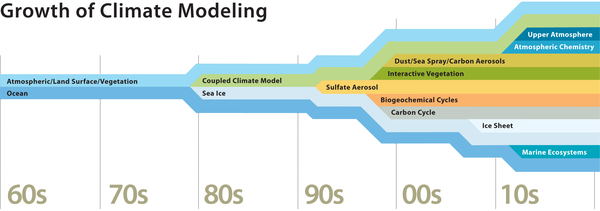
\includegraphics[width=0.58\textwidth]{evolution_of_climate_models}
  \caption{A growth and evolution timeline of climate models. The complexity of global climate models has increased enormously over the last four decades. The most powerful models, such as the \gls{cesm}, now have the capability of simulating a broad range of atmospheric processes, such as the impact of marine ecosystems on the atmosphere. \copyright \gls{ncar}.}
  \label{fig:growth_esm}
\end{wrapfigure}

\textbf{\glspl{esm}} have been rapidly evolving over the past decades (Fig.~\ref{fig:growth_esm}) due to growing computational resources. Over time the scope of the models has substantially broadened and the physical realism of the models has steadily increased, among others due improvements in resolution, grid types, parameterizations and couplers \parencite{AMS:Randall2018}. But this development comes at the cost of a complexity rivaling the real world and immense resources for computing. To predict the response of the Earth’s ecosystem in a changing climate and its feedback on the very same climate, it is important to update model parameterizations to reflect the  state-of-the-art scientific understanding of the underlying processes. From solving the Navier-Stokes equations of wind and waves several decades ago, \glspl{esm} came to represent even biotical process of soil microbial and fungi. But the more we learn the more do we know what is left unknown. At present missing links and knowledge gaps exist especially when it comes to the details of the complex interaction between terrestrial ecosystems and the atmosphere \textbf{\color{red}TODO: Add reference}. First analyses of \gls{cmip}~6 indicate a growing divergence between models \textbf{\color{blue}Added: \parencite{ESD:Tebaldi2021}}, in particular in the land and atmospheric components. Although this will not revoke our fundamental understanding of climate change, it still affects the reliability of model projections.\\

\textbf{The chemical composition of the atmosphere is complex} and the concentration of many important trace gases is highly variable in time and space and substantially influenced by natural and anthropogenic emissions. While increases in the concentrations of well-mixed greenhouse gases such as \ch{CO_2} and \ch{CH_4} are understood as the prime cause of anthropogenic climate warming, anthropogenic activity has also substantially affected the atmospheric concentration of many other chemical species, many of which have important radiative properties.

One of these chemical species is \textbf{ozone, an important trace gas in the lower and middle atmosphere}, and central to this proposal. In accordance with its effects and realm of occurence, we can distinguish the good (stratosphere), \emph{the bad} (troposphere), and \emph{the ugly} (ambient air) ozone throughout the atmosphere. Here we focus on the connection and feedback between the bad and ugly sides of ozone. After \ch{CO_2} and \ch{CH_4}, ozone is ranked third amongst the most potent climate forcers \parencite[Chapter 8]{IPCC2013}. It contributes to warming in the troposphere where it is produced as a secondary air pollutant in chemical cycles involving precursors such as \ch{CO} and \ch{NO_x} as well as hydrocarbons (\gls{voc}, \gls{bvoc}). Ozone is highly toxic and harmful to human health and many ecosystems. Model projections show diverse futures for surface ozone burdens under the \gls{rcp} scenarios, in sign and magnitude strongly dependent on changes in precursor emissions and climate \textbf{\color{red}TODO: Add references: general Reference} \parencites{JGR:Rieder2015}{AE:Rieder2018}{Nat:Skeie2020}. Projections of effects of future ozone air quality on human health and crop damage dependent on the level of ambition in both climate protection and precursor reduction \parencite{PTRS:Schneidemesser2020}.

Despite a successful reduction of precursors in recent years leading to a stagnation of the upward trend in tropospheric ozone concentrations, there are indications that \textbf{climate feedback on the ozone uptake by the land biosphere} can hamper reaching  air quality goals \parencite{NCC:Lin2020}. Under drought conditions, plants will limit their transpiration by closing their stomata, which regulate all of its gas exchange. At the same time, such stressed vegetation is emitting \glspl{bvoc}, an important precursor, and thus increasing ozone concentrations \ch{[O_3]} in ground-level air. As ozone uptake through plants’ stomata is considered one of the most effective removal pathways, stomatal closure under thermal stress will lead to a twofold penalty of climate change on vegetation and air quality. At present however, large uncertainties in non-stomatal removal remain \parencite{RG:Clifton2020}.

\begin{wrapfigure}[26]{R}[0pt]{0.5\textwidth}
  % R - floating; r - h! [narrow lines] <- reduce whitespace below [17]
  \centering
  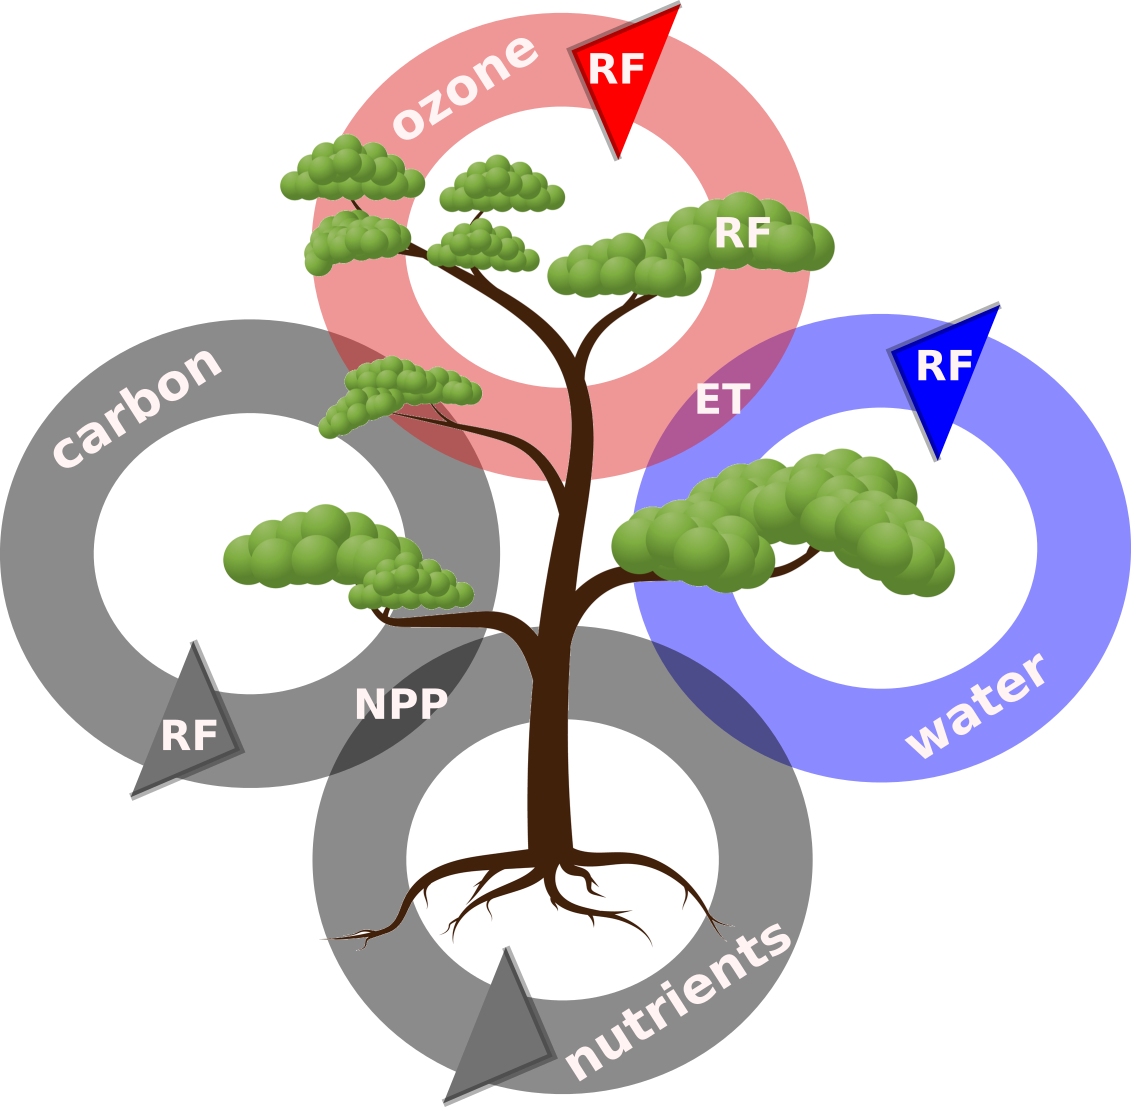
\includegraphics[width=0.48\textwidth]{ozone_es_scheme}
  \caption{Schematic view of the importance of ozone in \glspl{esm}. \textbf{\color{red}Ozone} inflicts damage to vegetation. Ozone affects photosynthesis negatively and hence \gls{npp} (\textbf{\color{darkgray}$\rightarrow$ carbon cycle}). Ozone affects opening and closing of stomata (positively and negatively) and hence \gls{et} of plants (\textbf{\color{blue}$\rightarrow$ water cycle}). Both affect the processing of nutrients (\textbf{\color{darkgray}$\rightarrow$ nutrient cycle}). Ozone damage on vegetation causes positive and negative feedback on tropospheric ozone concentrations and hence on air quality and \gls{rf} \parencite{Nat:Sitch2007}.}
  \label{fig:ozone_esm_scheme}
\end{wrapfigure}

Besides air quality considerations, \textbf{ozone interferes with the climate and Earth system} both directly and indirectly. Directly ozone affects the radiative forcing through its absorbance in both long and short wave bands and hence contributes to climate change. Indirectly ozone affects climate and air quality through ozone impacts on vegetation, which stand at the center of the proposed research. A high \gls{cuo} leads to considerably visible (e.g. necrosis, early senescence) and invisible damage (e.g. reduced photosynthesis, root growth) on vegetation \parencite{GCB:Mills2010}.

\textbf{\color{red}Ozone damage} reduces plant photosynthesis and stomatal conductance. As illustrated in Fig.~\ref{fig:ozone_esm_scheme}, ozone effects on vegetation interfere with several sensitive components of the Earth system. Ozone affects the \textbf{\color{darkgray}carbon cycle} through a reduced photosynthesis capacity and subsequent reduction in \gls{npp} and \gls{gpp}, which has consequences on the \textbf{\color{darkgray}nutrient cycle}. At the same time, physical damage will alter \gls{et} of the plant and hence the \textbf{\color{blue}water cycle}. Depending on the species and severity of damage both a reduction \parencite{Oe:Lombardozzi2012} or an increase (known as stomata sluggishness) have been reported \parencite{SR:Hoshika2015}. Accounting for ozone induced reduction of stomatal conductance and photosynthesis independently, \textcite{BGS:Lombardozzi2012} could improve model projections of changes in \gls{gpp} and transpiration on global scales.

In \textbf{our current understanding of photosynthesis at the plant physiological level}, maximum electron transport rate $\mathrm{J_{max}}$ and maximum carboxylation efficiency $\mathrm{V_{cmax}}$ are key parameters. Empirically it was found that ozone damage leads to a reduction of  $\mathrm{J_{max}}$ and $\mathrm{V_{cmax}}$ \parencite{EJA:Emberson2018}. Because the ratio $\mathrm{J_{max}}$:$\mathrm{V_{cmax}}$ is found to be constant (even under ozone exposure), first order effects of ozone induced damage can be modeled by a relative reduction in $\mathrm{J_{max}}$ or $\mathrm{V_{cmax}}$ alone. A simple linear relationship relates the relative reduction of $\mathrm{J_{max}}$ or $\mathrm{V_{cmax}}$ with the \gls{cuo} \parencites{BGS:Franz2017}{BGS:Franz2018}. \textcite{BGSD:Franz2020} showed that the impact of potential ozone damage on vegetation under climate change scenarios with explicit modeling on the plant physiological level has the potential to suppress projected gains in \gls{gpp} by increased nitrogen fertilization. These results however, have been based on a model without online atmospheric chemistry. \textbf{\color{red}TODO: Ueberleitung zum naechsten Absatz. \color{blue}Vorschlag: Offline coupling of a land model to ozone concentrations provided from another \gls{ccm} as often done lead to inconsistencies due to differing land use and surface roughness and hence dry deposition velocities between the models. Because the provided ozone concentrations from the \gls{ccm} are already in equilibrium with its own dry deposition scheme, a projected reduced uptake due to ozone damage would change the equilibrium concentration if coupled. To study the effects of ozone on vegetation and the feedback on air quality in the most consistent manner, a two-way coupling between land and atmosphere is essential.}\\

\important{Here, we aim to integrate state-of-the-art  process understanding at the vegetation level into a fully coupled \gls{esm} with coupled atmospheric chemistry and state-of-the-art nutrient limited carbon sequestration to study the effects of  ozone damage and thermal stress on vegetation and the resulting feedback on air quality  and climate.}

\section{Own contributions}
\label{sec:contrib}
The importance of ozone in the Earth system extends from large scales (stratospheric chemistry, dynamics, and radiation balance) to the smallest scales (damage on cellular level in plants). Following its trail, the applicant first studied \textbf{ozone depletion and future trends in the stratosphere} using the \gls{ccm} \gls{emac} model. In this respect the research activities primarily focused on future trends of biogenic brominated \gls{vsls} emitted from the ocean and the combined influence of sulfur aerosols \parencite{ACP:Falk2017}. In this study an increase of future ocean-atmosphere flux of brominated \gls{vsls} of $8-10\,\%$ compared to present day was found. A subsequent decrease in the tropospheric mixing ratios of brominated \gls{vsls} and an increase in the lower stratosphere are attributed to changes in atmospheric chemistry and transport and a reduced bromine impact on stratospheric ozone at the end of the 21st century was found  compared to the present day.

The episodic \textbf{\glspl{ode} from the polar spring-time boundary layer} which are associated with suddenly occurring high bromide abundances (bromine explosions) lead the applicants way to model development, precisely the implementation of a bromine release mechanism based on \textcite{ACP:Toyota2011} in the \gls{emac} model. Many aspects of the observed bromine enhancement and associated \glspl{ode} in both polar regions could be reproduced by the model including the applicants extension which paved the way for testing of bromine release mechanisms in a global model \parencite{GMD:Falk2018}.

Subsequently the applicant’s research focused on ozone at lower levels. As a major sink of ozone in the troposphere is dry deposition, the applicant turned her eye towards this problem and integrated the \textbf{variable uptake of ozone by the land biosphere} into the scheme of the Oslo \gls{ctm}~3 \parencite{GMD:Falk2019}. This work has substantially improved ozone dry deposition velocities and abundance to vegetated surfaces in the model, and drew attention to the need for more mechanistic descriptions of dry deposition to non vegetated surfaces.

In the following, the applicants work focused in detail on the representation of \textbf{ozone damage with a special focus on subarctic biomes} \textbf{\color{red}TODO: Add references (IPC Vegetation Taskforce Meeting 2021 and EGU conference contribution 2021)}. The analysis of \gls{do3se} model results revealed that standard parameters optimized for central Europe may lead to significant underestimation of damage inflicted to vegetation acclimated to subarctic climates. \textbf{\color{blue}Added text: The risk posed on subarctic biomes by the progressing climate change and a prolongation of the growing season may therefore be underestimated.}

Last but not least, the applicant studied at the smallest scales the \textbf{process-based impact of ozone on the leaf-level} and implemented the representation of ozone damage on nitrogen utilization in \gls{clm}~5.0 \textbf{\color{red}TODO: Remark first results presented at the \gls{cesm} landmodeling working group meeting 2021)} which is the foundation for the proposed development and analytical work in this project. This work indicated that the impact of ozone damage on \gls{gpp} strongly depends on the occurrence of the damage relative to the seasonal cycle of the vegetation.

\textbf{\color{red}TODO: Add remark that publications of these last two works are in preparation?}


\chapter{Aims \& hypothesis}
\label{c:aim_hyp}
%\glsresetall

The project \gls{odina} focuses on the process-based modeling of ozone induced damage on vegetation. To this end the applicant will implement a two-way coupling of ozone between the atmosphere and land-biosphere in a widely used global \gls{ccm}, the \gls{cesm}. \textbf{\gls{odina} studies the vegetations' feedback on near-surface to tropospheric ozone concentrations and will improve our process-level understanding of dry deposition effects on air quality and plant health.} The improved capabilities of \gls{cesm} including the \gls{odina} model will be demonstrated and effects of air quality regulations, and biosphere feedbacks on surface ozone air quality will be studied under the high emission \gls{ssp}~5. \gls{odina} will also enable the research team to study ozone impacts through vegetation on the global carbon cycle and water cycle, and thus ultimately climate.
The \gls{odina} project is guided by \textbf{five working hypotheses}: 

\begin{enumerate}
\itemsep0pt
\item Elevated ozone concentrations affect plant physiology via a reduction of the maximum electron transport rate and maximum carboxylation efficiency and a subsequent decreased stomatal conductance and photosynthesis. 
\item Reduced stomatal conductance will decrease ozone uptake by vegetation and hence diminish the dry deposition sink of ozone to the land biosphere. This will in turn act as a positive feedback increasing ground-level ozone concentrations in regions with damaged vegetation and thus degrading ambient air quality.
\item Decreasing stomatal conductance will further affect transpiration of plants implicating lower relative humidity and less cooling by latent heat. At the same time more water will remain in the soil.
\item A reduction of photosynthesis will affect the carbon sequestration and the terrestrial carbon sink, and hence diminish the removal of \ch{CO_2} from the atmosphere.
\item All described feedback mechanisms may increase surface air temperature and thus amplify local/regional temperature extremes.
\end{enumerate}

Guided by these hypotheses, the project team will specifically:
\begin{enumerate}
\itemsep0pt
\item Investigate the interaction between ozone and plant physiology and quantify on the one hand the degree of plant damage expected by elevated ozone concentrations, and on the other the anticipated increase in ozone burden due to a reduced dry deposition.
\item Quantify the effect of plant health on \gls{bvoc} emissions and subsequent effects on air quality.
\item Quantify the effect of reduced stomatal conductance and photosynthesis on carbon sequestration and \gls{et}, and thus indirect impacts of ozone on the climate forcing.
\end{enumerate}



\chapter{Innovation}
\label{c:innovation}
\textbf{The project \gls{odina} will improve our understanding of the two-way feedback between ozone and vegetation in the light of climate change}. The project targets key issues in international policies and efforts directed towards air quality and climate, but also, human health and food security.
The intended developments will \textbf{bridge the gap between state-of-the-art understanding of plant physiology and climate modeling}. 
Furthermore, an assessment of the contribution of plant health on the emission of \glspl{bvoc} may \textbf{pave the way for a wide range of new insights regarding aerosol formation} and related uncertainties under future climate conditions. This could provoke investigations into improving the \gls{bvoc} emission models, tying them more tightly to the physiological state of the vegetation in \glspl{esm}.

Although ozone-induced reduction of stomatal conductance and photosynthesis has been addressed previously (as reviewed in Section~\ref{sec:review}), ozone damage on vegetation has not been included into the nutrient cost driven photosynthesis on the process level and at the same time coupled to both atmosphere and atmospheric chemistry, in \gls{cesm}.
Such \textbf{extension of the \gls{cesm}} is a timely effort given the importance of the process and the extensive model user base. The \gls{cesm} user community extends worldwide, with about $4,000$ registered users in the support forum, and its importance for scientific discovery is reflected in about $3,000$ research and development papers published since 2009.

Without doubt, \textbf{new developments in such a widely used model will have a lasting impact on the climate and air quality research communities}. The proposed research will advance our modeling capacities and improve process representation beyond what is reflected in \gls{cmip}~5 or \gls{cmip}~6 generation models, and thus contribute to a \textbf{more complete understanding of surface air quality and more robust future projections}.



\chapter{Research methods \& model description}
\label{c:methods}
\textbf{Within \gls{odina}, we will apply and extend the latest release series of the \gls{cesm} and its components}, \gls{clm}~5 including \gls{bvoc} emissions (\gls{megan} model \parencite{ACP:Guenther2006}), \gls{cam}~6 with online (super-fast) chemistry (\gls{impact} model, \parencite{JGR:Rotman2004}). Below, we provide a brief technical account of the model components of \gls{cesm} most relevant to the planned work, \gls{clm} including \gls{megan}, and \gls{cam}. Subsequently we review the Lombardozzi model of ozone damage and close by introducing the new process oriented plant physiological model of ozone damage, developed by the applicant, including the planned integration into \gls{clm} that stands at the core of the \gls{odina} project.

%\begin{wrapfigure}[33]{R}[0pt]{0.5\textwidth}
  % R - floating; r - h! [narrow lines] <- reduce whitespace below [17]
\begin{figure}[!bh]
  \centering
  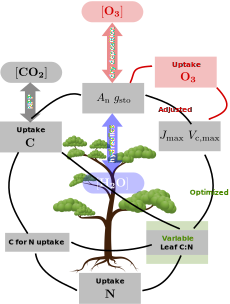
\includegraphics[width=0.72\textwidth]{ozone_luna_scheme} % 0.48
  \caption{Schematic view of the \gls{odina} model integration into \gls{clm}~5. Round boxes represent affected tropospheric chemistry (\gls{cam}-chem) and trace gas concentrations, e.g. \ch{[CO_2]}, \ch{[O_3]}, \ch{[H_2O]}. Annotated arrows denote the associated process. Squared boxes represent processes in the land model (\gls{clm}). Plants \textbf{\color{darkgray}invest carbon} to \textbf{\color{darkgray}take up nutrients}. A \textbf{\color{OliveGreen}variable \ch{C:N} ratio} at leaf level steers the optimization of electron transport ($\mathrm{J_{max}}$) and carboxylation rate ($\mathrm{V_{cmax}}$), which determine photosynthesis ($\mathrm{A_n}$) and stomatal conductance ($\mathrm{g_{sto}}$). $\mathrm{g_{sto}}$ controls transpiration and thus \textbf{\color{blue}plant hydraulics}. \textbf{\color{red}Ozone uptake} is determined by $\mathrm{g_{sto}}$ and reduces both $\mathrm{J_{max}}$ and $\mathrm{V_{cmax}}$. (own illustration)}
  \label{fig:ozone_odina}
\end{figure}
%\end{wrapfigure}

\vspace{-0.5\baselineskip}
\section{Community Earth System Model (CESM)}
\label{sec:cesm}
In \gls{clm}~5, \textbf{photosynthesis} (and hence the carbon cycle) \textbf{is tied to plant nutrient dynamics} (dark gray boxes in Fig.~\ref{fig:ozone_odina}) which incorporates the \textbf{\gls{fun}} model \parencites{GBC:Fisher2010}{JGR:Brzostek2014}{GCB:Shi2015}. The concept of \gls{fun} is that nitrogen uptake requires an investment of energy (e.g. carbon) and that there is a large number of potential sources of nitrogen available in the environment. The ratio of carbon invested to acquire nitrogen is therefore treated as a cost in the model. \gls{fun} calculates the rate of symbiotic nitrogen fixation for nitrogen that is passed directly to the plant, and subsequently delivered and incorporated as inorganic ammonium in the soil \parencite{GBC:Cleveland1999}, separately. Nutrient limitation is represented by a variable plant \ch{C:N} ratio which allows plants to adjust their \ch{C:N} ratio at the leaf level at the cost of nitrogen \parencite{JAMES:Ghimire2016}. The \textbf{\gls{luna}} model \parencites{STE:Xu2019}{GMD:Ali2016} finally links these processes with photosynthesis. To this end the \gls{luna} model calculates the photosynthetic capacity based on optimization of the use of leaf nitrogen under different environmental conditions. \textbf{Stomatal conductance} is based on this \textbf{nitrogen-limited photosynthesis} rather than on potential photosynthesis. The maximum stomatal conductance is obtained from the \textbf{Medlyn stomatal conductance} model \parencite{GCB:Medlyn2011} which is preferred over Ball-Berry-type models \parencite{BallBerry1987} for it’s more realistic behavior at low humidity levels (high vapor pressure deficit) \parencites{PR:Rogers2013}{NP:Rogers2017}.

As a \textbf{plant hydraulic stress} routine explicitly models water transport through the vegetation according to a simple hydraulic framework \parencite{JAMES:Kennedy2019}, stomatal conductance is also a function of prognostic leaf water potential and hence forced by transpiration. Plant water stress is calculated as the ratio of attenuated stomatal conductance to maximum stomatal conductance.

\textbf{Biogenic emissions} from vegetation are not directly integrated into the modeling framework described above but handled by \textbf{\gls{megan}} \parencite{ACP:Guenther2006}. \gls{megan} uses above canopy atmospheric forcing, e.g. solar radiation, temperature, and moisture, and \ch{[CO_2]} as input variables. \gls{megan} receives only \gls{pft} and \gls{lai} as vegetation input information, which can be either prescribed (\gls{sp} mode) or dynamic (\gls{bgc} mode). In \gls{clm}~5, \gls{megan}~version~2.1 \parencite{GMD:Guenther2012} is implemented. \gls{megan}~2.1 includes 147 chemical compounds which can be subset and grouped together (e.g. isoprene = pentane + hexane + heptane + tricyclene). In \gls{clm}, trapping of emissions inside of the canopy is explicitly disabled (i.e., escape efficiency set to 1).

In \textbf{\gls{cam}-chem}, \textbf{dry deposition} follows the resistance approach originally described by \textcites{AE:Wesely1989}{AE:Walcek1986} and updated sequentially \parencites{AE:Walmsley1996}{AE:Wesely2000}. All deposited chemical species are mapped to a weighted-combination of ozone and sulfur dioxide depositions to characterize their oxidation potential versus their solubility in water which is dependent on the effective Henry’s law coefficient of the species. All species in the mechanism are per default affected by dry deposition if deposition velocities are defined. The computation of \textbf{deposition velocities} (or resistances) ties \gls{cam}-chem to \gls{clm}. Dry deposition velocities vary with \gls{pft}. A grid-averaged velocity is computed as the weighted-mean over all land cover types. The impact from changes in land cover, land use or climate are thus directly reflected in the coupled model \parencite{GMD:Lamarque2012}. 

\section{Ozone damage in CESM}
\label{sec:ozone_damage}

\textbf{At present, ozone damage on vegetation is not reliably accounted for in \gls{cesm}}, due to a couple of technical reasons. First of all, the land surface model (\gls{clm}) as a stand-alone model would need at least a reliable global climatology of \ch{[O_3]} to integrate ozone damage in its default setup. Global ozone reanalysis (i.e. \gls{cam} reanalysis products of the \gls{ecmwf}) or satellite derived tropospheric ozone would be candidates but show, despite improvements in recent years, considerable biases compared to observations \parencites{GMD:Huijnen2020}{ACPD:Barten2020}. Though ozone climatologies based on older \gls{cesm} runs with \gls{cam} and \gls{clm} exist \parencite{ACP:Lamarque2010}, common caveats of such simulations with uncoupled ozone are:
\begin{enumerate}
\itemsep0pt
\item the inconsistency between the land surface (e.g. land use type, roughness length) used in the \gls{ccm} and the uncoupled land surfaces model with ozone damage functions, and
\item that ozone concentrations are not provided to \gls{clm} directly from the atmosphere and therefore mostly not in agreement with atmospheric abundances.
\end{enumerate}

Ozone damage in \gls{clm}~5 is based on the work of \textcite{Oe:Lombardozzi2012} which showed an effective decoupling of $A_\mathrm{n}$ and $g_\mathrm{sto}$ under high \gls{cuo}, with $g_\mathrm{sto}$ being less sensitive to ozone uptake. If taken into consideration this improves global projections of \gls{gpp} and transpiration considerably \parencite{BGS:Lombardozzi2012}, especially in tropical regions as also shown by \textcite{Nat:Sitch2007} and \textcite{ACP:Pacifico2015}. In this implementation, damage coefficients for $g_\mathrm{sto}$ and $A_\mathrm{n}$ are defined for coniferous, deciduous, and non-woody \glspl{pft}, respectively. \gls{cuo} can be regulated through an uptake threshold, further a healing factor is computed based on change in \gls{lai} (growth of new leaves). Technical limitations and issues of the current ozone damage module include its disconnection from the nutrient and carbon cost driven photosynthesis and compatibility with the plant hydraulic module. In particular, the order in which stomatal conductance is reduced under combined thermal and oxidative stress is not clearly constrained.

\textbf{Recent model development efforts led by the applicant have addressed some of the limitations listed above by integrating ozone damage on the process-level.} A linear relationship between \gls{cuo} and $\mathrm{J_{max}}$ in (both control and forced) experiments was deduced based on the body of peer reviewed research articles published in recent years. The \gls{odina} model integrates seamlessly into existing, scientifically validated modules in \gls{clm} (e.g. \gls{fun}, \gls{luna}). The integration of \gls{odina} into the existing framework of \gls{clm}~5 is schematically illustrated in Fig.~\ref{fig:ozone_odina}. \gls{odina} also builds on previous efforts by \textcites{BGS:Lombardozzi2012}{Oe:Lombardozzi2012}, leading to a comprehensive database of experimental data of ozone damage and an implementation of an ozone damage module in \gls{clm}~4 \parencite{BGS:Lombardozzi2013}. This database will be used for model evaluation of \gls{odina} as data are not included in the derivation of the linear relationship detailed above. One of the advantages of the \gls{odina} model is that it can be used to study ozone effects on the \ch{C:N} ratio  and thus the momentary plant health. While the nitrogen content of the leaves will likely stay unchanged, carbon uptake is reduced in response to ozone-induced damage to photosynthesis. Such disturbed \ch{C:N} ratio may trigger growth of new leaves.\\

A prime focus of this project is to establish the \textbf{coupling of \gls{clm}~5 to \gls{cam}-chem with respect to ozone through dry deposition} and evaluate the comprehensive two-way coupling of ozone-vegetation in the light of progressing climate change.


\chapter{Intended collaborations}
\label{c:collab}
The applicant will collaborate within the \gls{odina} project also closely with key developers of \gls{cesm} at \gls{ncar}/\gls{ucar} in Boulder, USA. Tasks in \gls{wp}2 (see Chapter~\ref{c:project_plan}) will be partially performed during a 3~months research stay at \gls{ncar}/\gls{ucar} hosted by Senior scientist Louisa Emmons (Atmospheric Chemistry Observations \& Modeling Lab) and Dave Lawrence section head of Climate \& Global Dynamics Lab and their teams (see \gls{loi}). Additional collaboration will include technical and scientific staff at the \gls{uio} (Norway), particularly \textbf{TODO: Add names}. 


\chapter{Project plan \& timeline}
\label{c:project_plan}
As specified in the call for the Lise-Meitner fellowship the project plan is aligned for a duration of 24~months. The project is divided into 5 tangible \gls{wp} (Fig.~\ref{fig:flowchart}) of varying duration. \gls{wp}0 (Management and mentoring) and \gls{wp}5 (Reporting and dissemination) are designed to run through the whole project duration of 24~months concomitantly (Fig.~\ref{fig:ganttchart}). \gls{wp}0 oversees the whole project and is central for the career development guided by the host institution. \gls{wp}0 has also a bi-directional component as mentoring and support is received by the applicant as well as given through co-supervision of master and PhD students. All communication, e.g. regular reporting to the \gls{fwf} and dissemination in the form of research papers, conference contributions, and public outreach activities , are bundled in \gls{wp}5. The scientific and technical work is assigned to \gls{wp}1-4. The technicality of the work packages is decreasing from \gls{wp}1 (mainly technical) - \gls{wp}4 (purely scientific) with expected increasing scientific throughput. \gls{wp}1 (Model integration) and \gls{wp}2 (Model coupling) are tightly interlinked with \gls{wp}3 (Model evaluation) spanning the whole duration of \gls{wp}1 and \gls{wp}2. \gls{wp}2 depends on the realisation of \gls{wp}1, and\gls{wp}4 depends on the completion of all previous substantial work packages (1-3). Important \glspl{ms} are specified in the \gls{wp} description below and marked  in Fig.~\ref{fig:ganttchart}. 
\glspl{ms} 1-3 mark the successful completion of \gls{wp}1-3, respectively. \glspl{ms} 4 and 5 refer to the successful completion of the subtask in \gls{wp}4 \glspl{ms} 3 and 5 also trigger reporting to the \gls{fwf}.

\begin{figure}
  \centering
  \subbottom[Flow chart]{%
    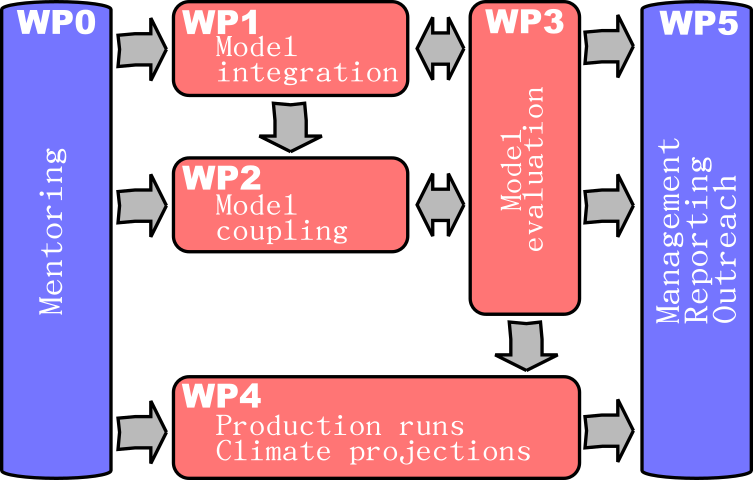
\includegraphics[width=0.48\linewidth]{wp_flow_chart}
  \label{fig:flowchart}}
  \subbottom[Gantt chart]{%
    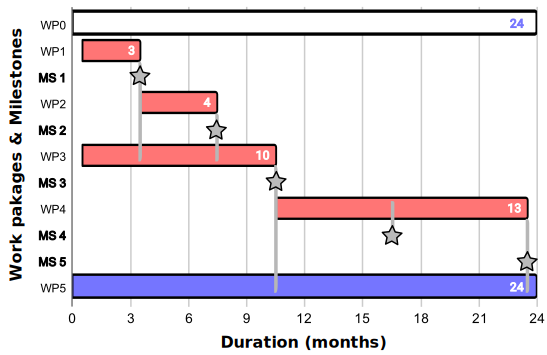
\includegraphics[width=0.48\linewidth]{gantt_chart}
  \label{fig:ganttchart}}
  \caption{\glspl{wp} as presented in this Section. \gls{wp}0 and \gls{wp}5 coordinate and communicate between the different \glspl{wp}m and therefore run during the whole duration of the project. Within \gls{wp}2 a three months research stay at \gls{ncar} lab in Boulder, COL, USA is planned. \gls{ms}~3 and 4 correspond to reporting to a funding agency (\gls{fwf}).
}
\end{figure}

\section{WP0 Management and mentoring}
\label{sec:wp0}
The management and mentoring \gls{wp}, as described above spans the entire project periode and includes a variety of bi-directional tasks in cooperation and with support of the faculty host and host institute at \gls{boku}. \gls{wp}0 is built upon the  core attributes of the Lise-Meitner fellowship  and shall enable the applicant to position herself as an emerging leader in land-atmosphere interactions, particularly the climate-vegetation-air quality nexus. During the start phase of the \gls{odina} project, \gls{wp}0 will ensure a smooth integration into the work environment at the host institute  and all aspects concerning technical, administrative and logistic support by the corresponding units of \gls{boku} (Task~0.1). The mid-phase is split into the development and honing of key skills for a future leadership role in Earth science (Task~0.2) and monitoring of the project progress (Task~0.3). Task~0.2 includes leadership and management training but also programs focusing on didactic skills, presentation techniques, public outreach formats, as well as contributions to  teaching and co-supervision of students. A detailed career development plan is presented in Section~\ref{sec:career}. In the end-phase \gls{wp}0 will initiate the preparation of follow-up proposals tailored to European and national funding schemes such as e.g. the \gls{fwf} Elise-Richter program or stand-alone projects (Task~0.4).

\subsection*{Work Package duration 24 months (months 1 to 24)}
\begin{enumerate}[start=1,label={T0.\arabic*}]
  \itemsep0pt
\item Getting started \hfill [month 1]
\item Career development \hfill [month 1 - 24]
\item Progress monitoring \hfill [month 1 - 23]
\item Follow-up projects \hfill [month 18 - 24]
\end{enumerate}

\section{WP1 Model integration}
\label{sec:wp1}
The model integration \gls{wp} will build on existing collaborations with technical and scientific staff at the \gls{uio} (Norway) and at \gls{ncar} in Boulder (USA) and include support by the scientific and technical team of the host institute at \gls{boku}, Vienna. Existing parts of the \gls{odina} model will be extended to describe our stateoftheart process understanding as accurately as possible. This will comprise
\begin{enumerate}
  \itemsep0pt
\item the inclusion of a state of stomata sluggishness,
\item to  consider a more explicit healing formulation for the \gls{odina} model (Task~1.1),  and
\item to deduce and update additional model parameters based on existing meta databases (Task~1.2).
\end{enumerate}
It is expected that the model output considering  active ozone damage will substantially differ between the updated (this proposal) and current model configuration (\gls{cmip}6). Initial cross-evaluation with data at global scales (coarse resolution model integration) and single site simulations (Task~1.3) following the \gls{cesm} standard procedures are likely to reveal the necessity for adjustment of additional free model parameters. In depth evaluation of individual parameters and results is subject to \gls{wp}3. In concert with \gls{wp}3 the \gls{wp}5 aims to present the  completed \gls{odina} model to the broad community on scientific meetings and within  a peer-reviewed model development paper (\gls{ms}~1 in Fig.~\ref{fig:ganttchart}).
\subsection*{Work Package duration 3 months (months 1 to 4)}
\begin{enumerate}[start=1,label={T1.\arabic*}]
  \itemsep0pt
\item Implementation of stomatal sluggishness and healing \hfill [month 1 - 2]
\item Deduction of additional parameters \hfill [month 2 - 3]
\item Initial model simulations and cross-evaluation \hfill [month 3 - 4]
\end{enumerate}

\section{WP2 Model coupling}
\label{sec:wp2}
Activities related to model coupling \gls{wp} will include a three month research stay at the \gls{ncar} lab in Boulder (USA) to both facilitate the technical work as well as build important networks for future work. A one-way coupling between the atmospheric chemistry component (e.g. \gls{cam}-chem) to the land-surface component (\gls{clm}) is achieved through the dry deposition implementation already in place in \gls{cesm}. The existing dry deposition scheme in \gls{cesm} will be evaluated concerning \gls{odina}. If necessary, the scheme will be improved and updated (Task~2.1). Two-way coupling will be achieved by propagating instantaneous ozone concentrations from the atmosphere through the coupler to the land component (Task~2.2). Technically this involves touching the model \gls{cesm} coupler infrastructure. The work on the coupling will be done in the most sustainable way during the planned research stay at \gls{ncar}. Potential infrastructure updates will be taken into consideration and integrated into the workflow. Initial tests and evaluation of the coupled model on coarse-grid global-scale as well as through  single site simulations are planned (Task~2.3). Detailed validation of the coupled model will be performed in coordination with \gls{wp}3 as in described in \gls{wp}1.

\subsection*{Work package duration 4 months (months 4 to 8)}
\begin{enumerate}[start=1,label={T2.\arabic*}]
  \itemsep0pt
\item Evaluation of the dry deposition scheme (improvement and update) \hfill [month 4 - 5]
\item Technically coupling \gls{cam}-chem ozone concentrations to \gls{odina} \\$\rightarrow$ research stay at \gls{ncar}/\gls{ucar} \hfill [month 5 - 6]
\item Perform model  tests of the coupling algorithm \hfill [month 6 - 8]
\end{enumerate}

\section{WP3 Model evaluation and update of model parameters}
\label{sec:wp3}
The evaluation of the updated model is an integral part of \gls{wp}1 and \gls{wp}2 and spans the whole duration of both \gls{wp}. Data for evaluation will be collected from FLUXNET sites with associated ground level ozone observations, e.g. \gls{airbase} (Task~3.1). Based on the collected data, the initial integration and validation tests are complemented and completed with more in depth evaluation for the selected sites (Task~3.2) and on global scales (Task~3.3). Model parameters  (e.g. $\mathrm{J_{max}}$0 in \gls{luna}, \glspl{pft}) will be adapted and adjusted for changes in the model baseline of, e.g. in terrestrial and vegetation carbon pools, inflicted ozone induced damage on photosynthesis and stomatal conductance (Task~3.4). A model evaluation paper after successful evaluation is pursued in coordination with \gls{wp}5 (\gls{ms}3). The model development and evaluation paper could be synthesized into one if necessary.

\subsection*{Work Package duration 10 months (months 1 to 11)}
\begin{enumerate}[start=1,label={T3.\arabic*}]
  \itemsep0pt
\item Collection of evaluation data \hfill [month 1 - 3]
\item Site level evaluation \hfill [month 3 - 6]
\item Global scale evaluation \hfill [month 6 - 11]
\item Update model parameters \hfill [month 3 - 11]
\end{enumerate}

\section{WP4 Production runs and climate projections}
\label{sec:wp4}
Upon successful implementation of \gls{wp}1-3 work on \gls{wp}4 is initiated. Within this final research work package production runs with climate projections will be performed. It is planned to perform at least one long term \gls{cmip} style ($1850-2100$) coupled model simulation (Task~4.1). As the highest tropospheric ozone abundances are expected for a low mitigation scenario with high anthropogenic greenhouse gas emissions and simultaneous substantial methane release from permafrost regions \parencites[e.g.][]{JGR:Rieder2015}{AE:Rieder2018}, thus \gls{ssp}~5 is selected as a future scenario. Additional simulations following other \glspl{ssp} are planned but depend on the workload at \gls{vsc} and thus cannot be guaranteed to be fully complete within the 24~month project timeline. Results will be compared with existing \gls{cmip}~6 reference simulations of \gls{cesm} to study the combined effects of climate and ozone feedback on vegetation in a coupled \gls{esm} (Task~4.2). Of special interest are implications on future surface ozone abundance and air quality indices along with induced plant damage and effects on the carbon cycle, e.g. expected reduction in \gls{gpp} with respect to reference simulations. The focus herein lies on populous and highly industrialized regions, e.g. Europe, East Asia, North America.

\subsection*{Work Package duration 13 months (months 11 to 24)}
\begin{enumerate}[start=1,label={T4.\arabic*}]
  \itemsep0pt
\item Run \gls{cesm} coupled of climatological timescales (\gls{ssp}5) \hfill [month 11 - 17]
\item Study climate and vegetation impact on surface ozone abundance \hfill [month 17 - 24]
\end{enumerate}

\section{WP5 Reporting and dissemination}
\label{sec:wp5}
\gls{wp}5 acts as an umbrella for reporting to the funding agency (\gls{fwf}) and dissemination to scientific and lay audiences. \gls{wp}5 spans the whole project duration and is effectively the coordinating and reporting hub for \gls{wp}1--4. Science communication (Task~5.1) is further divided into publications, e.g. research papers, conference contributions, and public outreach. Public outreach will include among others contributions to popular science blogs or presentations to the general public. Dissemination using social media platforms such as twitter will be considered if applicable. In close interaction with \gls{wp}0 and under guidance by the host institution, targeted networking activities are planned (e.g. conferences, workshops, professional networks) (Task~5.2). The submission of the final report to the funding agency (\gls{fwf}) is officially concluding \gls{wp}5 (Task~5.3) although several additional papers are expected to emerge from the project results which will be submitted past official completion.

\subsection*{Work Package duration 24 months (months 1 to 24)}
\begin{enumerate}[start=1,label={T5.\arabic*}]
  \itemsep0pt
\item Science communication \hfill [month 3 - 24]
\item Networking \hfill [month 1 - 24]
\item Submit final report  to funding agency (\gls{fwf}) \hfill [month 23 - 24] \textbf{\color{red}TODO: Abklaeren, wann dieser faellig ist.}
\end{enumerate}


\chapter{Research-related qualifications of the researchers involved}
The applicant, \textbf{Stefanie Falk}, is a physicist by training. Her postdoctoral stations included the \gls{kit} and the \gls{uio}. Her curiosity about the complex and important role of ozone in the atmosphere led her from studying its chemical depletion in the stratosphere and polar boundary layer to its formation and removal processes by the land biosphere. Interdisciplinary work has been a cornerstone in her work to improve the understanding and push the development of current numerical models of the Earth system forward. In particular, she has been working on \gls{ccm} using the \gls{emac} model. Her work was related to future trends of stratospheric ozone, biogenic brominated \gls{vsls}, and the influence of sulfur aerosols. During her engagement at \gls{kit}, she also implemented a bromine release mechanism from snow and studied ozone depletion in the Arctic boundary layer. Identifying dry deposition as a key issue for both future air quality as well as climate, she committed to studies on the effects of ozone on vegetation in her latest work at \gls{uio}. From ozone formation and dry deposition on global and regional scales, her focus shifted later to process-based impact modeling at the leaf level and improvements of subarctic biomes. Her work resulted in scientific publications and conference contributions both nationally and internationally. She gladly participates in public outreach, at \gls{uio} through public lectures and popular science blogs in the Norwegian language. She is a member of the \gls{dpg} and the professional body of the environmental section in the \gls{dpg}, \gls{yess} community, and the \gls{eswn}.\\

\textbf{Harald Rieder} is full professor and head of the institute of meteorology and climatology at the University of Natural Resources and Life Sciences, Vienna. He is an expert in chemistry-climate connections. His research is centered on the climate-air quality-health nexus and combines numerical models with observational data sets from both ground-based networks and remote sensing platforms. He has led and extensively contributed to studies unravelling the effect of changes in climate, ambient meteorology, and anthropogenic emissions on surface pollution as well as the effects of atmospheric composition changes for climate at the surface and at upper atmospheric levels. Prof. Rieder serves among others as board member of the Austrian Centre for Climate Change and Member of the \gls{isac} Atmosphere Working Group.


\chapter{Ethical, safety-related, or regulatory aspects}
No other research of ethical, security-related or regulatory issues is foreseen. 


\chapter{Sex-specific \& gender-related issues}
The project does not raise any sex-specific and gender-related issues.


\chapter{Information on the research institution \& career development}
\label{c:info_dev}
\section{Added value to be expected from this collaboration}
The \gls{odina} project shows excellent fit with the research priorities of the host institution. The \gls{boku}, Vienna is an international leader in environmental sciences with research priorities comprising the preservation and development of the environment and quality of life, management of natural resources and the environment and safeguarding food and health. Prof. Rieder’s group at \gls{boku} focuses on chemistry-climate connections, particularly the effects of changes in atmospheric composition on climate and air quality across temporal and spatial scales. Within the framework of \gls{odina} Dr. Falk and the host group would be the first to develop a fully coupled ozone module within the \gls{cesm} and apply it to study impacts and feedback mechanisms for plant health and air quality. Given the diversity of research within the \gls{boku} community that focuses on plant physiology and plant health the model development and research activities within \gls{odina} will pave the road for manifold research endeavors ahead, and thereby create a lasting resource for \gls{boku} and the Austrian research landscape. Furthermore, the updated model version will increase the portfolio of contributions of the Rieder group to international activities within the framework of \gls{igac} activities such as \gls{toar}-2 and \gls{ccmi}-2.

\section{Importance of the project for the academic and research reputation of the applicant and her career development}
The \gls{odina} project will allow the applicant to pursue her research interests and spearhead the inclusion of coupled ozone chemistry in one of the widest used community earth system models. Thereby she will be able to position herself as an emerging leader in the field of coupled modelling with focus on land-atmosphere interactions, particularly the climate-vegetation-air quality nexus. Interaction through model development and application with the \gls{cesm} core team and \gls{igac} community will expand and strengthen her peer network. The scientific and technical support of the host group and broader \gls{boku} community will provide an ideal environment for project implementation. The mentoring and career development program accompanying this proposal will prepare Dr. Falk for an academic career ahead.

\section{Career Plan}
\label{sec:career}
In her research Dr. Falk strives to advance our understanding of causes and effects of changes in the chemical composition of the Earth’s atmosphere. To this end she applies state-of-the-art earth system models and contributes to their continuous development to improve the process level understanding and reduce uncertainties and biases in model projections. Dr. Falk aims to establish herself as an independent researcher with focus on the climate-air quality-health nexus and strives to achieve a permanent academic position either via a tenure-track faculty line or a senior scientist appointment. The proposed Lise-Meitner Fellowship is an important stepstone towards this goal.\\
The research framework of the fellowship project \gls{odina} allows Dr. Falk to follow her research interest and strengthen her scientific and technical portfolio to propel her career. Dr. Falk will spend her Lise-Meitner fellowship in Prof. Rieder’s group at the \gls{boku}, guaranteeing a stimulating research environment and ideal project support infrastructure. Prof. Rieder and his team focus on chemistry-climate connections, particularly ozone, and embedment in the \gls{boku} community will provide rich opportunities for interaction with research teams focusing on plant health and biosphere-atmosphere interaction. Including a module for coupled ozone chemistry between the atmosphere and land-surface components of \gls{cesm} Dr. Falk will provide an important extension to one of the widest used earth system models and provide rich opportunities for colleagues focusing on ambient air quality, ozone dry deposition and ozone plant damage and plant physiology. Given the broad impact of the model extension and opportunity to explore processes and feedbacks in the atmosphere-land system the \gls{odina} project will allow Dr. Falk to establish herself as an emerging leader in the field of land-atmosphere interaction.\\
The model development activities of \gls{odina} will link Dr. Falk with the core development team of the CESM model at the National Centre for Atmospheric Research in Boulder, CO, USA. The connection to NCAR’s Atmospheric Chemistry Observations \& Modeling Lab and Climate \& Global Dynamics Lab will be fostered through a 3-month research stay in the first year of the project. The \gls{odina} project will embed Dr. Falk also in the TOAR-2 and CCMI-2 activities of the International Global Atmospheric Chemistry (IGAC) Project and thereby substantially expand her professional network.\\
Throughout the project the interaction between the Dr. Falk and Prof. Rieder will focus on all aspects related to the mentees career development and the overall progress of the research project. To this end they will meet for discussions on a weekly basis. These meetings will focus on the one hand on project status, opportunities or challenges emerging and scientific findings, on the other on recently published research highlights in the field, emerging funding and employment opportunities, as well as upcoming conferences or trainings. Prof. Rieder will provide dedicated support to Dr. Falk throughout the project. He will provide guidance and counseling in all scientific and professional aspects, introduce Dr. Falk to his network of peers and promote her as guest speaker for institute seminars and conferences. He will further provide guidance in the leverage of research results for high-profile publication formats and the effective dissemination of research outcomes via traditional media and online platforms. Besides Prof. Rieder, Dr. Falk will obtain mentoring by Dr. Mayer (\gls{boku}-Met) and other peers in the Earth Science Women’s Network.\\
As an affiliate of \gls{boku} Dr. Falk will have access to a wide range of training and career development programs offered by the university. These include among others leadership training and didactic training as well as a variety of courses tailored to strengthen skills in project acquisition and project management and the preparation of application packages for tenure-track or staff scientist positions or the preparation of a habilitation thesis. Dr. Falk will be further assisted through \gls{boku}’s programs within the framework of the Postdoc Coaching Group and individual career coaching sessions. During her fellowship at \gls{boku} Dr. Falk will also gain experience in the mentoring and co-advising of undergraduate and graduate students within Prof. Rieder’s group and be supported in dissemination and outreach activities by the university media and public relations office.\\
To ensure continued funding after the end of the Liese-Meitner funding period Prof. Rieder and the \gls{boku} office for research support, innovation \& technology transfer will support Dr. Falk in the development of applications to national and European Union research programs. Furthermore to ensure further collaboration Prof. Rieder and his team will and include Dr. Falk in their own applications submitted to these funding schemes.     


%\vspace*{5cm}
\vfill
\vspace{5cm}

\begin{minipage}{.4\textwidth}
  \hrulefill
  
  \hspace*{0mm}\phantom{}Dr. Stefanie Falk
  
  \hspace*{0mm}\phantom{}Applicant
\end{minipage}%
\hfill
\begin{minipage}{.4\textwidth}
  \hrulefill
  
  \hspace*{0mm}\phantom{}Prof. Harald Rieder
  
  \hspace*{0mm}\phantom{}Co-Applicant
\end{minipage}




%\backmatter
\appendix
%Print the glossary
\printglossaries

\newpage
\printbibliography[env=bibliography]

\end{document}
